\documentclass[letterpaper,12pt]{article}
\usepackage{times}
\usepackage[utf8]{inputenc}  %acentos
\usepackage[spanish]{babel}
\usepackage{graphicx}
\graphicspath{{Images/}}
\usepackage{geometry}
\geometry{left=18mm, right=18mm, top=21mm, bottom=21mm} %tamaño del área
\usepackage{ucs}
\usepackage{amsmath,amsfonts,amsthm}    %paquetes matemáticos
\usepackage[lofdepth, lotdepth]{subfig}  %Colocar varias figuras
%\usepackage{subfigure}
\usepackage{unitsdef}     %Presentación correcta de unidades 
\usepackage{float}
\usepackage{ragged2e,afterpage}
\usepackage{wrapfig}
\usepackage{booktabs}
\pagestyle{plain}
\pagenumbering{arabic}
\usepackage{lastpage}
\usepackage{fancyhdr}
\pagestyle{fancy}
\usepackage[export]{adjustbox}
\usepackage{listings}
\usepackage{placeins}

\lhead{Control I}
\rhead{Polos y Zeros: Método de Inspección}
\lfoot{Depto. de Ingeniería Electrónica}
\cfoot{\thepage\ de \pageref{LastPage}}
\rfoot{Instituto Tecnológico de Morelia}

\title{Instituto Tecnológico de Morelia\\{\small DIVISIÓN DE ESTUDIOS PROFESIONALES\\DEPARTAMENTO DE INGENIERÍA ELECTRÓNICA\\CONTROL I\\\vspace*{0.2in} REPORTE DE PRÁCTICA 2}\\ {Polos y Zeros: Método de Inspección }}

\author{
	%\textbf{EQUIPO 6A} \\\\
	\textbf{INTEGRANTES:}
	\\Luis David Herrera Chávez   14121093 
	\\ \hspace{-1.7cm}Ivan Marín Paredes  14121097					 \\\\ 
	\textbf{Semestre:} \\ Agosto-diciembre 2017\\\\ 
	\textbf{Profesor:} \\ M.C Gerardo Marx Chávez Campos\\\\\\\\}

 %$---------------------------------------------------------------
 
 \newcounter{introducción}
 \setcounter{introducción}{0}
 \newenvironment{introducción}
 { 
 	\begin{center}
 		\begin{minipage}[t]{500 pt}
 			\vspace{5mm}
 			\emph{\textbf{}}
 			\\[-4.25 mm]
 			\line(1,0){500}
 			\\
 		}
 		{
 			\normalsize
 			\\[-2mm]
 			\line(1,0){500}
 			\\[0.5cm]
 			
 		\end{minipage}
 	\end{center}
 
 }
 
 \begin{document}
 	\begin{figure}[t]
 		\centering
 		
\includegraphics[scale=0.9]{Header}
 		
 	\end{figure}
 	\maketitle
 	
 	\thispagestyle{empty}
 	
 	
 	\newpage
 	
 	\section*{INTRODUCCIÓN}
 	\addcontentsline{toc}{section}{Resumen}
 	
 	\begin{introducción}
 		En esta sesión de laboratorio se hace uso práctico sobre lo que se vio en las horas de teoría respecto al comportamiento de un sistema y su función de transferencia. En este caso se hace el análisis de un circuito eléctrico el cual es un sistema de primer orden. Lo que se hizo para su análisis fue por inspección estimar su función de transferencia y posteriormente se hizo algebraicamente. Para la simulación se utilizó LTSpice para simular el circuito y posteriormente, se pasó al laboratorio para  corroborar lo obtenido en la simulación. 
 	\end{introducción}
 
   
   \section*{PARTE I}
   El circuito a analizar en esta práctica es el que se muestra en la siguiente imagen.
   
   \begin{figure}[h]
   	\centering
   	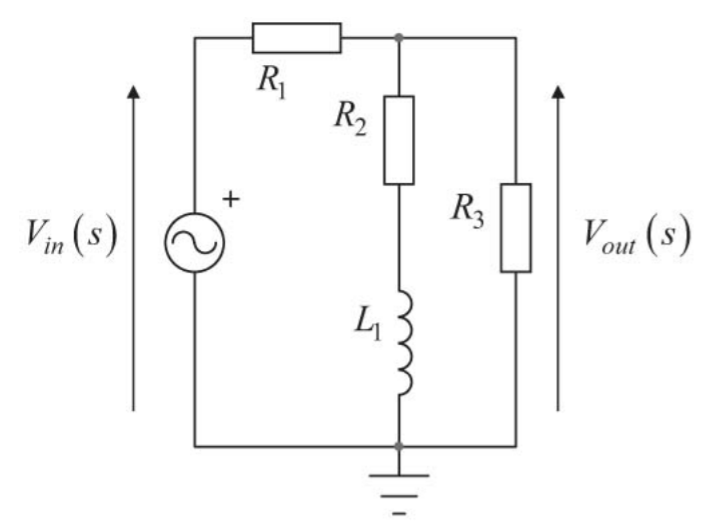
\includegraphics[scale=0.6]{circuito}
   	\caption{Circuit for part 1}
   
   \end{figure}
\subsection*{INSPECCIÓN}
Como se observa en la figura 1, el circuito tiene conectado en serie una resistencia y un inductor, para la ganancia en corriente directa se sabe que los inductores se cortocircuitan. Esto nos dice que la salida del circuito se puede calcular mediante un divisor de tensión ya que se obtiene una resistencia equivalente ($R_2$ y $R_3$) conectada en serie con $R_1$. Como la ganancia es igual al voltaje de salida entre el voltaje de entrada, simplemente se despeja $V_i$ del divisor de voltaje obteniendo así :
$$\frac{V_{out}(s)}{V_{in}(s)}= \frac{\frac{R_2R_3}{R_2+R_3}}{R_1+\frac{R_2R_3}{R_2+R_3}}$$
\\
Ya que se obtuvo el término $G_0$, hace falta calcular los polos y ceros. Para esto se presta atención en la rama que contiene al inductor debido a que es el elemento que cambia su impedancia de acuerdo a la frecuencia en la que está trabajando. Basta con decir que $R={\omega}L$. Relacionando esto con nuestro circuito se tiene que:
$$\omega_{z1}=\frac{R_2}{L}$$
donde $\omega_{z1}$ es el cero del sistema.\\
Para calcular ahora el polo del sistema, se abre el circuito donde está el inductor y se calcula su resistencia equivalente, obteniendo así, algo parecido al cero obtenido:
$$\omega_{p1}= \frac{R_eq}{L}$$ \\

Con los datos obtenidos y como se sabe que la función de transferencia es de la forma:
$$H(s)= G_0\frac{1+s/\omega_{z1}}{1+s/\omega_{p1}}$$
se obtiene la siguiente función de transferencia:
$$H(s)=\frac{\frac{R_2R_3}{R_2+R_3}}{R_1+\frac{R_2R_3}{R_2+R_3}}\frac{1+Ls/R_2}{1+Ls/R_{eq}}$$

\subsection*{ALGEBRAICO}
Para obtener la expresión de la ganancia se toma en cuenta lo que se menciona anteriormente. Esto es, que en corriente directa el inductor se pone en corto circuito como se muestra en la siguiente imagen.\\

\begin{figure}[h]
	\centering
	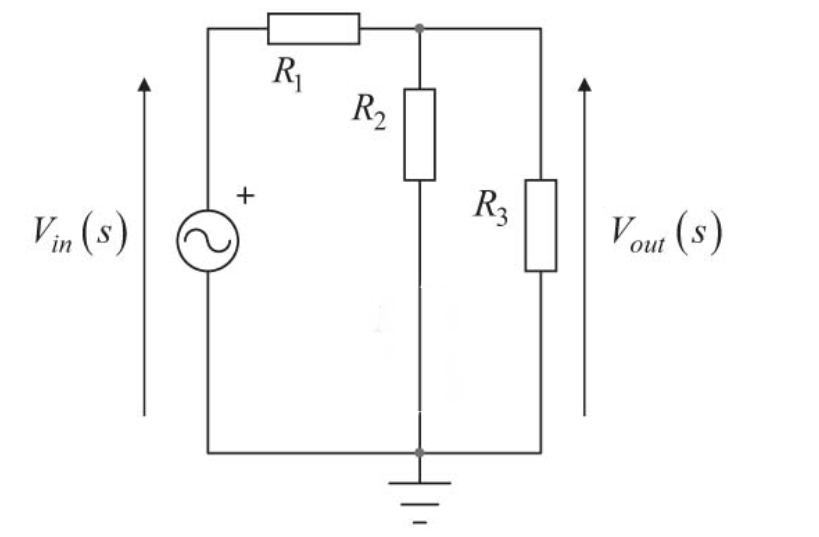
\includegraphics[scale=0.5]{F_2}
	\caption{Circuito equivalente en DC}
\end{figure}

Lo primero que se hace es calcular el paralelo de $R_2$ con $R_3$:
$$R_{eq}=\frac{R_2R_3}{R_2+R_3}$$
\\
Una vez que se tiene la resistencia equivalente, se tienen dos resistencias en serie y, gracias a esto, el voltaje de salida se puede obtener mediante un divisor de voltaje de la siguiente manera:

$$V_{out}(s)= \frac{R_{eq}}{R_1+R_{eq}}V_{in}(s)$$
\\
Sustituyendo $R_{eq}$ se obtiene:
$$\frac{V_{out}(s)}{V_{in}(s)}= \frac{\frac{R_2R_3}{R_2+R_3}}{R_1+\frac{R_2R_3}{R_2+R_3}}$$
\\
como $\frac{V_o}{V_i}= G_0$:
$$G_0=\frac{\frac{R_2R_3}{R_2+R_3}}{\frac{R_1(R_2+R_3)+R_2R_3}{R_2+R_3}}$$

$$G_0=\frac{R_2R_3}{R_1(R_2+R_3)+R_2R_3}$$

Ya que se tiene la expresión de la ganancia se requieren calcular los polos y ceros. Primero se inicia con el cero de la función: si se analiza la rama en la que se tiene el inductor, se tiene que:
$$R_2+SL=0$$ \\
Dividiendo la expresión entre $R_2$ se tiene:
 $$1+\frac{SL}{R_2}=0$$ \\
 Donde se sabe que $$\frac{S}{\omega_{z1}}$$
 \\
 Por lo tanto se tiene que:
 $$\omega_{z1}=\frac{R_2}{L}$$\\\\\\
 \newpage
 
 Para encontrar el polo observe la siguiente figura:
 
\begin{figure}[!h]
	\centering
	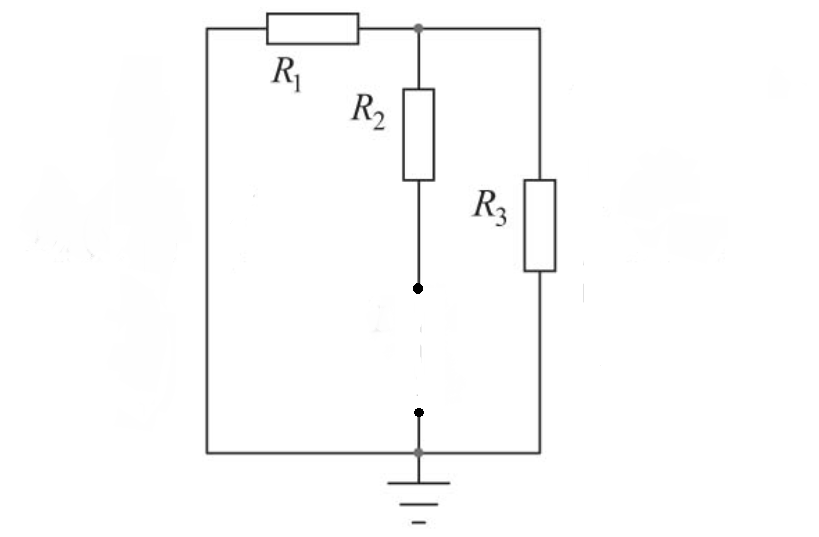
\includegraphics[scale=0.5]{F_3}
	\caption{Circuito abierto}
\end{figure}

En la figura se observa que la resistencia equivalente puede ser calculada de la siguiente forma:
$$R_{eq}=R_2+R_1{\parallel}R_3$$

$$R_{eq}=R_2+\frac{R_1R_3}{R_1+R_3}$$
$$R_{eq}=\frac{R_1(R_2+R_3)+R_2R_3}{R_1+R_3}$$ \\
Ya que se conoce la resistencia equivalente y sabiendo que $\omega_{p1}$ se calcula como el inverso de tau ($\tau$): $\omega_{p1}=\frac{1}{\tau}$ y además:
$$\tau=\frac{L}{R_{eq}}$$\\
Se tiene que:
$$\omega_{p1}=\frac{R_{eq}}{L}$$\\
Sustituyendo el valor de $R_{eq}$:
$$\omega_{p1}=\frac{\frac{R_1(R_2+R_3)+R_2R_3}{R_1+R_3}}{L}$$
$$\omega_{p1}=\frac{R_1(R_2+R_3)+R_2R_3}{L(R_1+R_3)}$$

Ya que se obtuvo la ganancia, los polos y los ceros, se puede escribir la función de transferencia de la siguiente forma:

$$H(s)=\frac{R2\parallel R3}{R1+(R2\parallel R3)}\frac{1+\frac{SL}{R2}}{1+\frac{SL}{R2+(R1\parallel R3)}}$$

$$H(s)=\frac{R_2R_3}{R_1(R_2+R_3)+R_2R_3}\frac{1+\frac{SL}{R_2}}{1+\frac{SL}{R_2+R_1\parallel R_3}}$$
\section*{PARTE II}
A continuación se realiza un análisis en tiempo y frecuencia del circuito anterior, realizado en el simulador de circuitos LTI Spice obteniendo los siguientes resultados:
\begin{figure}[H]
	\centering
	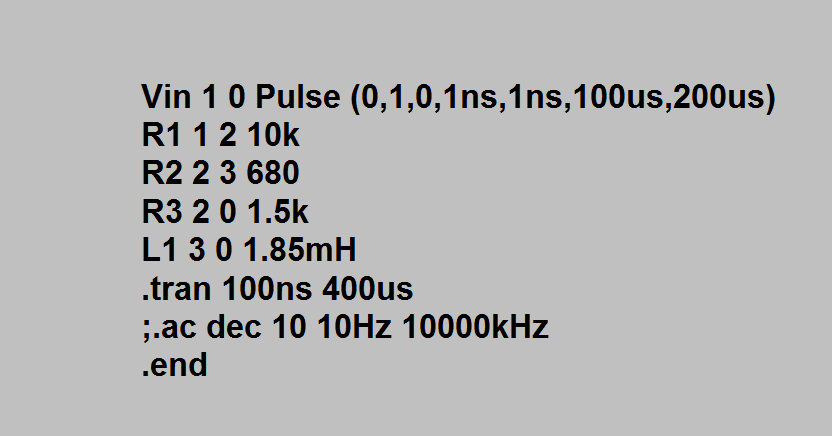
\includegraphics[scale=0.7]{SimTiempo}
	\caption{Código generado para el análisis en tiempo.}
	\label{CTiempo}
\end{figure}
\begin{figure}[H]
	\centering
	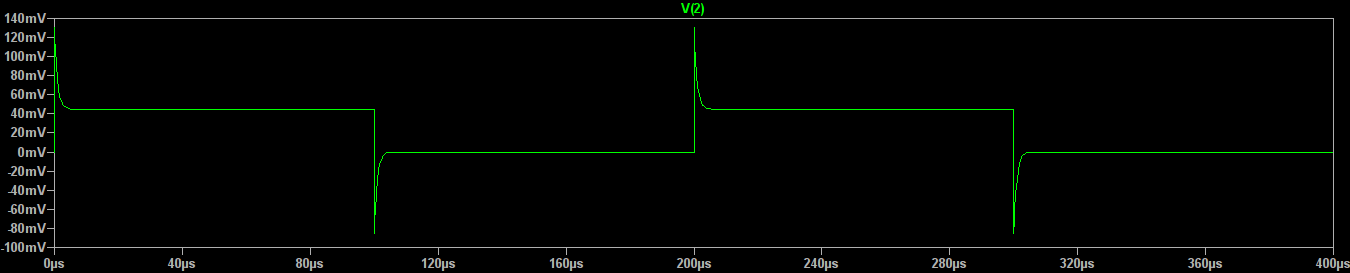
\includegraphics[scale=0.6]{SimTiempoGrafica}
	\caption{Gráfica de $V_{OUT}$ para el análisis en tiempo.}
	\label{CTiempoG}
\end{figure}
\begin{figure}[H]
	\centering
	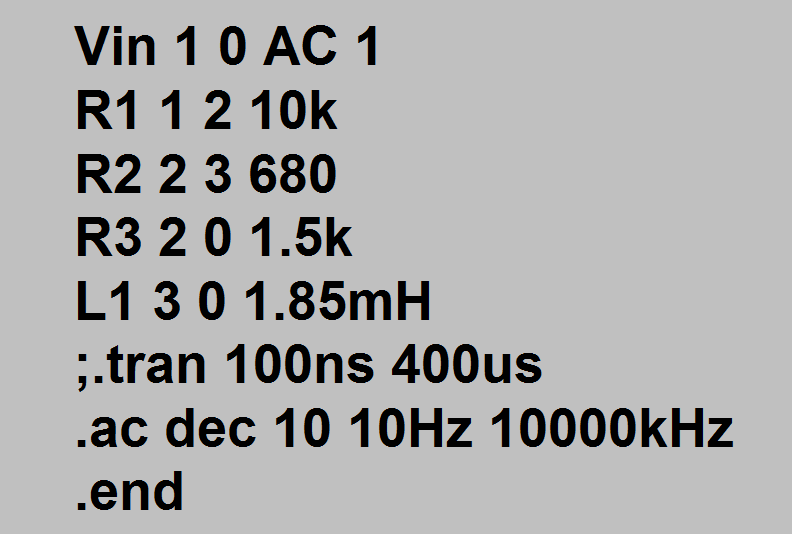
\includegraphics[scale=0.7]{SimFrecuencia}
	\caption{Código generado para el análisis en frecuencia.}
	\label{CFrecuencia}
\end{figure}
\begin{figure}[H]
	\centering
	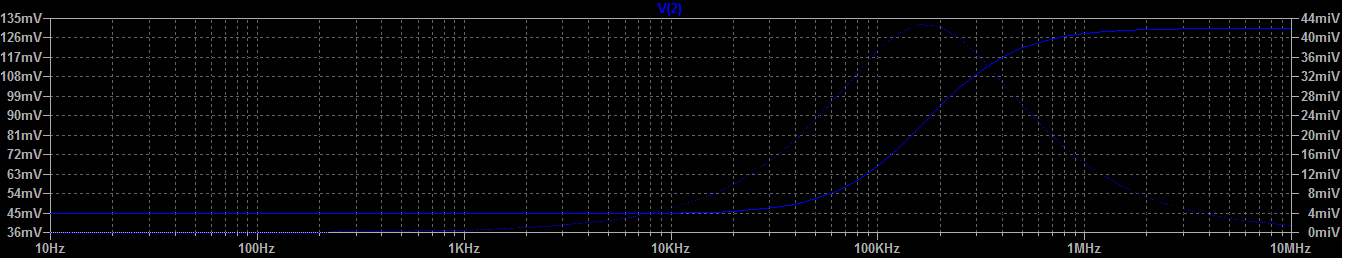
\includegraphics[scale=0.6]{SimFrecuenciaGraficaVoltaje}
	\caption{Gráfica de $V_{OUT}$ para el análisis en frecuencia contra voltaje.}
	\label{CFrecuenciaV}
\end{figure}
\begin{figure}[H]
	\centering
	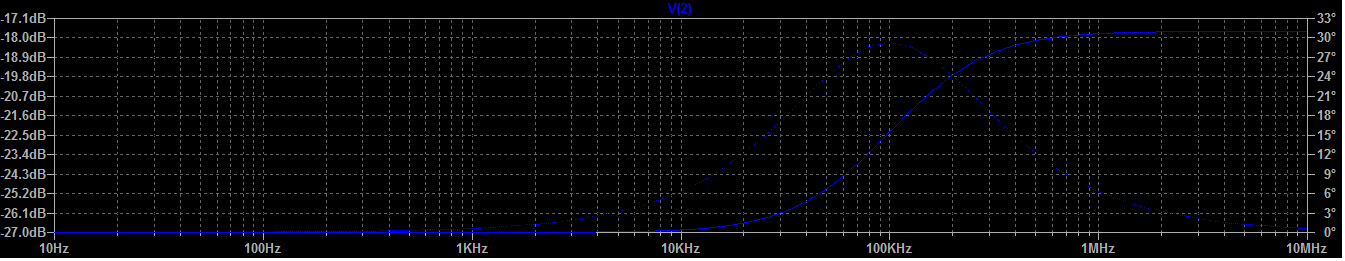
\includegraphics[scale=0.6]{SimFrecuenciaGraficaBode}
	\caption{Gráfica de $V_{OUT}$ para el análisis en frecuencia contra ganancia.}
	\label{CFrecuenciaB}
\end{figure}
\section*{PARTE III}
En esta parte de la práctica se realizo la implementación del circuito de la parte 1, se realizo el análisis de la respuesta en el tiempo para lo que se obtuvo la gráfica como se muestra en la figura \ref{ATiempo}: 
\begin{figure}[H]
	\centering
	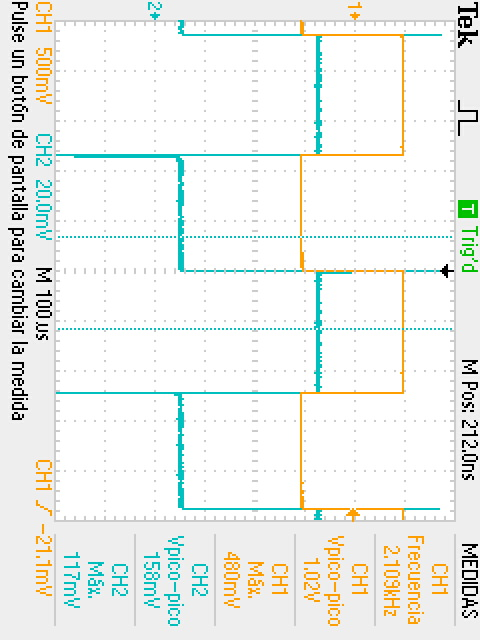
\includegraphics[scale=0.7,angle=90]{TEK0002}
	\caption{Análisis en el tiempo de $V_{out}$.}
	\label{ATiempo}
\end{figure}
\justify
Calculamos la $\tau$ del circuito, primero obteniendo la resistencia equivalente de acuerdo a los valores de las resistecias de nuestro circuito:$$R_{EQ}=\frac{10k\Omega*1.5k\Omega}{10k\Omega+1.5k\Omega}+680\Omega$$ $$R_{EQ}=1.98k\Omega$$
\\
Con la cual se calculo $\tau$ de acuerdo a los valores de nuestro inductor y resistencia equivalente: 
$$\tau=\frac{L}{R_{EQ}}=\frac{1.85mH}{1.98k\Omega}$$ 
$$\tau=932nS$$ 
\\
Al medir físicamente la  $\tau$ en el osciloscopio se muestra mediante la siguiente figura \ref{MTao}:
\begin{figure}[H]
	\centering
	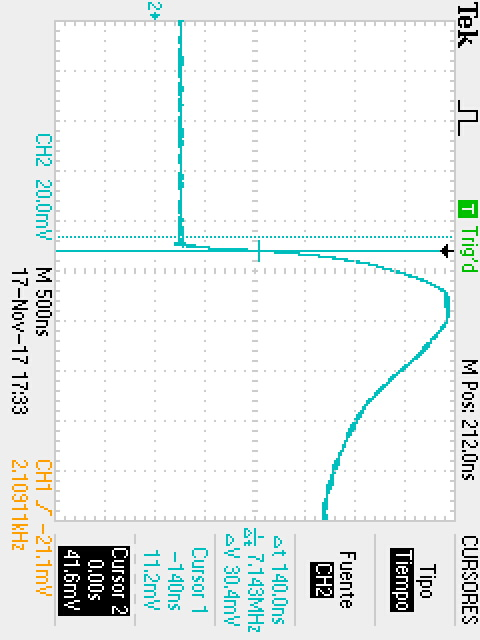
\includegraphics[scale=0.7,angle=90]{TEK0001}
	\caption{Medición del $\tau$ del sistema.}
	\label{MTao}
\end{figure}
\justify
Como se puede observar en la figura anterior el $\tau$ del sistema es $140nS$.
\\
Posterior al análisis de la respuesta en el tiempo, se procedió a hacer un análisis de su respuesta en frecuencia, mediante un barrido en frecuencia, obteniendo los siguientes datos y sus respectivas gráficas:
\begin{table}
	\caption{Barrido en Frecuencia }
	\centering
	\begin{tabular}{|r|r|}	
		\hline
		\multicolumn{1}{|l|}{Frecuencia} & \multicolumn{1}{l|}{Vout(Vpp(mV))} \\ \hline
		1.00E+06 & 144 \\ \hline
		9.00E+05 & 150 \\ \hline
		8.00E+05 & 160 \\ \hline
		7.00E+05 & 180 \\ \hline
		6.00E+05 & 200 \\ \hline
		5.00E+05 & 220 \\ \hline
		4.00E+05 & 240 \\ \hline
		3.00E+05 & 244 \\ \hline
		2.00E+05 & 220 \\ \hline
		1.00E+05 & 156 \\ \hline
		9.00E+04 & 148 \\ \hline
		8.00E+04 & 144 \\ \hline
		7.00E+04 & 136 \\ \hline
		6.00E+04 & 132 \\ \hline
		5.00E+04 & 124 \\ \hline
		4.00E+04 & 116 \\ \hline
		3.00E+04 & 112 \\ \hline
		2.00E+04 & 108 \\ \hline
		1.00E+04 & 106 \\ \hline
		9.00E+03 & 108 \\ \hline
		8.00E+03 & 108 \\ \hline
		7.00E+03 & 108 \\ \hline
		6.00E+03 & 108 \\ \hline
		5.00E+03 & 104 \\ \hline
		4.00E+03 & 104 \\ \hline
		3.00E+03 & 104 \\ \hline
		2.00E+03 & 104 \\ \hline
		1.00E+03 & 104 \\ \hline
		900 & 104 \\ \hline
		800 & 104 \\ \hline
		700 & 104 \\ \hline
		600 & 104 \\ \hline
		500 & 104 \\ \hline
		300 & 104 \\ \hline
		200 & 104 \\ \hline
		100 & 104 \\ \hline
	\end{tabular}
	\label{Barrido en Frecuencia}
\end{table}
\begin{figure}[H]
	\centering
	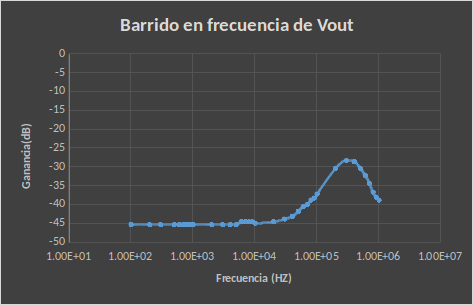
\includegraphics[scale=0.7]{Grafica1}
	\caption{Barrido en Frecuencia en Db.}
	\label{Grafica1}
\end{figure}
\begin{figure}[H]
	\centering
	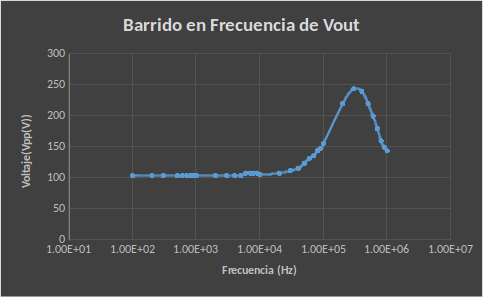
\includegraphics[scale=0.7]{Grafica2}
	\caption{Barrido en Frecuencia en mV.}
	\label{grafica2}
\end{figure}
\section*{Conclusiones}
En la realización de esta practica se comprobó la modificación del factor Q de acuerdo a los valores de resistencias que se elegían, este aspecto se resalto sobre todo en la simulación del circuito, el cual nos hacia un poco mas abrupta la manera en que llega a la frecuencia de corte, ademas de ver la variación en los decibeles, buscando así mediante la simulación los mejores valores de las resistencias para construir  el filtro físicamente.  
\\
Al implementar el circuito físicamente no se obtuvieron los resultados esperados, teniendo una previa idea de su comportamiento debido a la simulación antes realizada. Este fenómeno se puede atribuir principalmente al inductor, debido a que no estaba diseñado para funcionar a altas frecuencias ya que esta formado con un núcleo de aire, el cual no trabaja bien a altas frecuencias. Para obtener una respuesta mas acorde a la simulación se tiene que construir tu propio inductor que trabaje a frecuencias mas elevada, así se podría obtener una curva  mas cercana a la simulada.\\
Su frecuencia de corte se podrían considerar dos diferentes por su comportamiento, la primer a $90kHz$ y la segunda a $900kHz$, por lo que se podria decir que se esta comportando como un filtro pasa banda, cuando lo que se esperaba de su comportamiento era un filtro pasa altas.
   
 \end{document}